% India's electricity in 2047: forecast from the two challenge datasets and a robust regional strategy.
% Build: latexmk -pdf main.tex      (presentation)
%        latexmk -pdf reader.tex    (reader's edition: a note page after every slide)
% Every number comes from data/*.csv (copies of outputs/, run of 16 Nov 2026) or a cited source.
\documentclass[aspectratio=169,10pt,t]{beamer}
\usetheme{India2047}
\ifdefined\readeredition
  \setbeameroption{show notes}
\fi

\usepackage[style=numeric-comp,sorting=none,backend=biber,maxbibnames=3,giveninits=true,url=true,doi=true]{biblatex}
\addbibresource{refs_data.bib}
\IfFileExists{refs_web.bib}{\addbibresource{refs_web.bib}}{}
\IfFileExists{refs_academic.bib}{\addbibresource{refs_academic.bib}}{}
\renewcommand*{\bibfont}{\fontsize{6.6}{7.8}\selectfont}

\title{India's electricity in 2047}
\subtitle{A back-tested forecast from India's own data and a robust regional generation strategy}
\author{Ayush Kumar \and Devendra Umbrajkar \and Sai Anirudh Guttapati \and Gaurav Choudhary \and Tathagata Ghosh}
\institute{Indian Institute of Science, Bengaluru}
\date{ExxonMobil INNOTHON 2026}

\newcommand{\twh}{\,TWh}
% Styles with parameters must live outside frames.
\tikzset{
  lab/.style={font=\fontsize{7.5}{9}\selectfont,text=ink,fill=white,inner sep=1pt}}
\newcommand{\up}[1]{\textcolor{good}{\bfseries #1}}
\newcommand{\down}[1]{\textcolor{signal}{\bfseries #1}}
\newcommand{\qa}[2]{\emph{``#1''}\ #2\par\smallskip}

\begin{document}

% =====================================================================  1
{
\setbeamertemplate{footline}{}
\begin{frame}[plain]
\begin{tikzpicture}[remember picture,overlay]
  \fill[navy] (current page.south west) rectangle (current page.north east);
  \begin{scope}[shift={(current page.south west)}]
    \goldenmotif{8.30}{1.25}{4.45}
  \end{scope}
  \node[anchor=north west,text width=7.3cm,align=left,text=white] at ($(current page.north west)+(0.75,-0.85)$) {%
    {\fontsize{8.5}{10}\selectfont\color{white!70}ExxonMobil INNOTHON 2026\quad\textbar\quad Midpoint review}\par\vspace{4mm}
    {\phiM\bfseries India's electricity in 2047}\par\vspace{2.5mm}
    {\fontsize{12}{14.5}\selectfont\color{white!90}A back-tested forecast from India's\\ own data and a robust regional plan}};
  \node[anchor=south west,text width=7.3cm,align=left,text=white] at ($(current page.south west)+(0.75,1.0)$) {%
    {\phiL\bfseries 4{,}894\,{\phiS TWh}}\par\vspace{0.5mm}
    {\fontsize{8.5}{10.2}\selectfont\color{white!80}median utility generation in FY2047-48\\ 2.88$\times$ FY2023-24\\ about 5,540\,TWh including captive plants}};
  \node[anchor=south west,text width=15cm,align=left,text=white!70,font=\fontsize{6.5}{8}\selectfont] at ($(current page.south west)+(0.75,0.40)$) {%
    Ayush Kumar \textbullet{} Devendra Umbrajkar \textbullet{} Sai Anirudh Guttapati \textbullet{} Gaurav Choudhary \textbullet{} Tathagata Ghosh\quad\textbar\quad Indian Institute of Science, Bengaluru};
\end{tikzpicture}
\note{%
\textbf{Message.} One number anchors the talk: India's utilities must generate about 4,894\,TWh in FY2047-48 (median), 2.88 times the 1,698\,TWh of FY2023-24 (4.5\% a year). Adding captive plants at today's share gives about 5,540\,TWh.\par\medskip
\textbf{Scope, said once and kept.} The core forecast is NPP utility generation in fiscal years, labelled by start year (2047 = FY2047-48). Captive plants sit outside NPP and are shown beside the forecast, never inside it.\par\medskip
\textbf{Design.} The motif is a golden rectangle with its nested squares and spiral. The same ratio sets every column split (0.605\,:\,0.365) and the type steps (10, 16.2, 26.2, 42.4\,pt). Numbers are the largest element on every slide.\par\medskip
\textbf{Evidence.} NPP generation FY2023-24 (dashboard chart); median of 4,194,304 scenarios, \texttt{outputs/forecast\_national\_regional.csv}; captive layer, \texttt{outputs/core\_comparison.csv}.}
\end{frame}
}

% =====================================================================  2
\begin{frame}{The answer on one page}
\begin{columns}[T,onlytextwidth]
\column{0.32\textwidth}
  \stat{4,894\twh}{median FY2047-48, utility scope (P10--P90 3,553--6,829); 5,540 with captive plants}{\cite{npp_dashboard,organiser_dataset}}
\column{0.32\textwidth}
  \stat{4.0\%}{largest holdout error ($-$4.0\% FY2024-25, +1.6\% FY2025-26), years never used in fitting}{\cite{npp_18col}}
\column{0.32\textwidth}
  \stat{0\twh}{unmet at the median with the robust plan, also \up{45\,bn USD/yr cheaper}}{\cite{e47_repo}}
\end{columns}
\vspace{0.5mm}
\begin{columns}[T,onlytextwidth]
\column{\gA\textwidth}
  \card{\linewidth}{\fontsize{8}{9.7}\selectfont
  \textbf{\color{navy}What we found.} \textbf{Income growth sets the size:} 1.5 points of growth per person moves 2047 by \textbf{+32\%} or \textbf{$-$24\%}. \textbf{Need is not where generation is:} the West makes 36\% of today's conventional generation but needs 27\% of 2047's. \textbf{Land and build rate bind:} the base plan is \down{28\,TWh short} at the median and \down{1,958} at P90; the robust plan closes the median gap at \up{188 instead of 233\,bn USD/yr}.}
\column{\gB\textwidth}
  \card{\linewidth}{\fontsize{7.8}{9.4}\selectfont
  \textbf{\color{navy}Built on}\\[0.6mm]
  NPP generation, FY2006-07 to 2025-26\\
  state population, GSDP (Renewable India)\\
  4.2 million simulated futures\\
  36 states, 5 grid regions\\
  least-cost optimiser, 7 corridors}
\end{columns}
\evidence{Model outputs \texttt{forecast\_national\_regional.csv}, \texttt{holdout.csv}, \texttt{sensitivity\_2047.csv}, \texttt{presets.csv}, \texttt{core\_comparison.csv} \cite{e47_repo}; NPP \cite{npp_dashboard,npp_18col}; organiser data \cite{organiser_dataset}; captive plants \cite{cea_general_review_2025}.}
\note{%
\textbf{Message.} Three numbers carry the case: the size of the need (4,894\,TWh), the credibility of the method (holdout errors of $-$4.0\% and +1.6\% on two years the model never saw) and the decision (a robust plan with no shortfall at the median that also costs less).\par\medskip
\textbf{Numbers to remember.} Base plan: 233\,bn USD/yr, 1,364\,Mt CO$_2$, 70.0\% non-fossil, 28\,TWh unmet at P50, 1,958 at P90. Robust plan: 188\,bn USD/yr, 1,114\,Mt, 76.5\%, 0 at P50, 1,067 at P90 (\texttt{presets.csv}, scenario Base).\par\medskip
\textbf{Likely questions.}\par
\qa{Is this compliant with the two-dataset rule?}{Yes: the forecast is estimated only on NPP generation and the organiser's population and GSDP. Literature supplies one prior (urbanisation) and the captive share; both are switchable (slide 4).}
\qa{Why is the robust plan cheaper?}{It unlocks cheap solar by relaxing land and build-rate limits that push the base plan onto nuclear and coal.}}
\end{frame}

% =====================================================================  3
\begin{frame}{Aligned with ExxonMobil's view of the energy future}
\framesubtitle{More energy for a growing, more prosperous India, with lower emissions}
% Slide 3: alignment with ExxonMobil's Global Outlook 2026 (quotes verified, see research_notes.md).
\begin{columns}[T,onlytextwidth]
\column{\gA\textwidth}
{\fontsize{7.5}{9}\selectfont
\renewcommand{\arraystretch}{1.28}
\begin{tabular}{@{}>{\raggedright\arraybackslash}p{0.46\linewidth}@{\hspace{2.5mm}}>{\raggedright\arraybackslash}p{0.50\linewidth}@{}}
\textbf{\color{muted}ExxonMobil says} & \textbf{\color{navy}Our answer for India}\\[-1mm]
\midrule
\itshape ``\ldots the need for more energy \emph{and} lower emissions'' \cite{exxon_outlook_2026_summary}
& Generation rises \textbf{2.18$\times$} by 2047, while the robust plan cuts power-sector CO$_2$ from about 1,480 to \textbf{920\,Mt}.\\
\itshape ``Growing global population and prosperity have been the biggest factors driving increased demand'' \cite{exxon_outlook_2026_intro}
& Population, income and urbanisation drive our forecast, learned from \textbf{153 countries}.\\
\itshape ``\ldots no single pathway can be reasonably predicted'' \cite{exxon_outlook_2026_summary}
& We simulate \textbf{4.2 million} futures and choose the plan that holds in \textbf{9 of 10}.\\
\itshape ``Lead industry in innovations that advance modern living and a net-zero future'' \cite{exxon_who_we_are}
& The coal that remains in 2047 sits at a few hundred large stations: a ready market for \textbf{carbon capture} \cite{exxon_ccs}.\\
\bottomrule
\end{tabular}}
\column{\gB\textwidth}
\vspace{1mm}
\stat{$\approx$42\%}{of the world's energy-demand growth to 2050 comes from India in ExxonMobil's own projection}{}
\vspace{2.5mm}
{\fontsize{8}{9.8}\selectfont\color{ink}
India's share of world energy demand rises from \textbf{7.5\%} to \textbf{11.2\%} by 2050 \cite{exxon_outlook_2026_data}. World electricity demand grows about 65\% by 2050 \cite{exxon_outlook_2026_summary}; India's generation requirement grows 118\% by 2047.\par\vspace{1.5mm}
ExxonMobil's technology centres are in Bengaluru, as are we \cite{exxon_india_operations}.}
\end{columns}
\evidence{ExxonMobil Global Outlook 2026: executive summary pp.\,2 and 13, introduction, data workbook \cite{exxon_outlook_2026_summary,exxon_outlook_2026_intro,exxon_outlook_2026_data}; corporate vision \cite{exxon_who_we_are}; the 42\% share is our arithmetic on ExxonMobil's data file (31.0 of 73.3 quadrillion BTU of growth).}
\note{%
\textbf{Why this slide.} The jury is from ExxonMobil. Their Outlook frames the challenge as ``more energy \emph{and} lower emissions'' and says that ``no single pathway can be reasonably predicted''. Our work answers both halves for India's electricity and replaces a single pathway with a probability distribution and a plan that is robust across it.\par\medskip
\textbf{The 42\% figure.} In ExxonMobil's 2026 data workbook, India's energy demand rises from 46.6 to 77.6 quadrillion BTU (2025--2050) while world demand rises by 73.3; 31.0/73.3 $\approx$ 42\%. This is our arithmetic on their data, not their wording; say so if asked.\par\medskip
\textbf{Carbon capture.} Even the robust plan keeps about 21\% coal in 2047 (about 940\,TWh). ExxonMobil describes itself as a global leader in carbon capture and storage; large, concentrated coal stations are the natural first market.\par\medskip
\textbf{All quotes} are verbatim from the sources cited and listed with page numbers in \texttt{docs/beamer/research\_notes.md}.}

\end{frame}

% =====================================================================  4
\begin{frame}{The core forecast uses only the two challenge datasets}
\begin{columns}[T,onlytextwidth]
\column{\gB\textwidth}
  \card{\linewidth}{\fontsize{8}{9.7}\selectfont
  \textbf{\color{navy}1. Two datasets for the core.}\\ NPP energy generated; Renewable India population and GSDP. Its capacity columns are never read.\\[1.2mm]
  \textbf{\color{navy}2. Literature only as priors and limits.}\\ Excess urbanisation ($\gamma$), captive share (+13.2\%, shown beside), potentials, costs. Each can be switched off.\\[1.2mm]
  \textbf{\color{navy}3. Requirement $\neq$ production.}\\ Need follows people and income; production follows resources. Corridors connect them.}
\column{\gA\textwidth}
\centering
\begin{tikzpicture}[x=1cm,y=1cm,
  box/.style={rounded corners=2pt,fill=tint,minimum height=7mm,inner sep=1.4mm,font=\fontsize{7.2}{8.6}\selectfont,align=center,text width=2.25cm},
  core/.style={box,draw=navy,line width=0.9pt},
  lit/.style={box,draw=muted,dashed,line width=0.6pt,fill=white},
  arr/.style={-{Latex[length=2mm]},line width=1pt,draw=navy3}]
  \node[core] (d1) at (0,2.2) {\textbf{NPP generation}\\FY2006-07 to 2023-24};
  \node[core] (d2) at (0,1.05) {\textbf{Population, GSDP}\\(Renewable India)};
  \node[lit]  (d3) at (0,-0.15) {Urbanisation prior\\$\gamma$ (literature)};
  \node[box,fill=navy,text=white,text width=1.9cm] (req) at (2.95,1.05) {\textbf{Requirement}\\by region, TWh};
  \node[box,fill=navy,text=white,text width=1.9cm] (prod) at (2.95,-1.45) {\textbf{Production}\\by region, source};
  \node[lit,text width=2.45cm] (r1) at (5.95,0.85) {Solar, wind, offshore\\(NISE, NIWE)};
  \node[lit,text width=2.45cm] (r2) at (5.95,-0.3) {Hydro, nuclear sites\\(CEA, DAE)};
  \node[lit,text width=2.45cm] (r3) at (5.95,-1.45) {Coal fleet, costs\\(CEA, IEA, SECI)};
  \node[anchor=south,font=\fontsize{7}{8}\selectfont\bfseries,text=navy] at (d1.north) {core: two challenge datasets};
  \node[anchor=south,font=\fontsize{7}{8}\selectfont\bfseries,text=muted] at (r1.north) {limits from literature};
  \draw[arr] (d1) -- (req); \draw[arr] (d2) -- (req); \draw[arr,dashed,draw=muted] (d3) -- (req);
  \draw[arr] (r1.west) to[out=180,in=30] (prod.north east); \draw[arr] (r2.west) to[out=180,in=10] (prod.east); \draw[arr] (r3.west) -- (prod.east |- r3.west);
  \draw[arr,draw=signal,line width=1.4pt] (prod) -- node[left,font=\fontsize{7.2}{8.6}\selectfont,text=signal,align=right]{transfers,\\7 corridors} (req);
\end{tikzpicture}
\end{columns}
\evidence{Competition rule (kickoff, 13 Nov 2026). Core data \cite{npp_dashboard,npp_18col,organiser_dataset}; urbanisation prior \cite{liddle2013population,shahbaz2016role,holtedahl2004residential}; captive share \cite{cea_general_review_2025} (Table 1.6); limits \cite{mnre_restats_2425,cea_hydro_status,cea_nep_vol2}; \texttt{outputs/india\_fit.csv}; column audit \texttt{docs/data\_audit.md} \cite{e47_repo}.}
\note{%
\textbf{Message.} The only parameter estimated for the 2047 total is the income elasticity, from the two challenge datasets. Literature supplies priors and limits only, each switchable.\par\medskip
\textbf{Evidence.} NPP dashboard chart and CEA 18-column reports on NPP; organiser file read for Population and GSDP only (\texttt{docs/data\_audit.md}).\par\medskip
\textbf{Likely questions.}\par
\qa{Is this compliant with the two-dataset rule?}{The estimation is. Population and urban paths to 2047 are literature growth paths, which the rule allows. $\gamma = 0$, the pure two-dataset run, gives 4,647\,TWh (5\% lower). We have asked for a ruling on the prior and the captive layer.}
\qa{Why not installed capacity?}{It is banned as a metric, and capacity is not energy. GW potentials only cap generation, through stated capacity factors.}
\qa{What about captive?}{224\,TWh in FY2023-24 (13.2\% of NPP utility generation), outside NPP; shown beside the forecast at that share.}}
\end{frame}

% =====================================================================  5
\begin{frame}{What is new: five advances over the state of practice}
% Slide 5: advances over the state of practice, each with evidence.
{\fontsize{7.4}{8.9}\selectfont
\renewcommand{\arraystretch}{1.3}
\setlength{\tabcolsep}{4pt}
\begin{tabular}{@{}>{\raggedright\arraybackslash}p{1.85cm}>{\raggedright\arraybackslash}p{4.0cm}>{\raggedright\arraybackslash}p{4.0cm}>{\raggedright\arraybackslash}p{3.85cm}@{}}
\toprule
& \textbf{\color{muted}State of practice} & \textbf{\color{navy}This work} & \textbf{\color{good}Evidence}\\
\midrule
\textbf{Demand outlook} & One demand path per year from the 20th Electric Power Survey, plus a flat +5\% case \cite{pib_nep_2023,powerline_nep_scenarios_2023}
 & A full probability distribution from 4.2 million consistent futures & 2047: P5 3,351, median 4,536, P95 5,606\,TWh\\
\textbf{Long-range method} & 2036--47 values ``by extrapolating\ldots with the application of suitable growth rates'' \cite{powerline_20th_eps_2022}
 & Saturation learned from 153 countries' generation \cite{yoo2010electricity,wolfram2012energy}, anchored on India & Fitted to 2010: 0.6\% error in 2025; trend extrapolation 29\%\\
\textbf{Scenarios} & Conditional scenarios: ``None of the individual WEO scenarios should be regarded as a forecast'' \cite{iea_weo_scenarios}
 & Every input carries a probability; model weights come from the back-test \cite{bates1969combination} & Uncertainty attributed: urbanisation $\approx$13\%, population $\approx$9\%\\
\textbf{Planning} & A plan built around one demand path \cite{pib_nep_2023}
 & Robust plan, stress-tested at the 90th-percentile requirement \cite{lempert2003shaping} & Unmet at P90: 447 $\to$ \textbf{0\,TWh}; cost $-$36\,bn USD/yr\\
\textbf{Speed and audit} & Studies rerun in batch & 4.2 million futures in 30\,ms on a GPU; identical inputs on CPU and GPU \cite{salmon2011parallel} & 7.5\,ms vs 22.7\,s on one CPU thread; parity within 0.2\%\\
\bottomrule
\end{tabular}}
\evidence{Practice: CEA National Electricity Plan 2022--32 and 20th EPS \cite{pib_nep_2023,iep_20th_eps_2022,powerline_20th_eps_2022}; IEA scenario framing \cite{iea_weo_scenarios,iea_weo2025_scenarios_commentary}. Our results: \texttt{outputs/} tables \cite{e47_repo}.}
\note{%
\textbf{How to present.} Read the middle column as our contribution and the right column as the proof. Each row is a claim the jury can check in the dashboard or the repository.\par\medskip
\textbf{Fair framing of the state of practice.} The CEA plan is a carefully built bottom-up study; its long-range values (2036--37, 2041--42) come from extrapolation with growth rates, and its demand side has a single base path plus a +5\% sensitivity. The IEA explicitly says its scenarios are not forecasts. ExxonMobil's Outlook is a single ``most probable'' projection. None of these attaches probabilities to electricity demand; that is the gap we fill.\par\medskip
\textbf{Saturation literature.} Cross-country studies find per-capita electricity demand flattening with income (Yoo and Lee 2010) and S-shaped appliance adoption as incomes rise (Wolfram, Shelef and Gertler 2012); our Gompertz model is consistent with both.}

\end{frame}

% =====================================================================  6
\begin{frame}{From two datasets to a regional plan in six steps}
\vspace{1.5mm}
\centering
\begin{tikzpicture}[
  stepbox/.style={rounded corners=3pt,fill=tint,inner sep=2mm,anchor=north west},
  arr/.style={-{Latex[length=2.2mm]},line width=1.4pt,draw=signal}]
  \foreach \i/\x/\y/\t/\b/\n in {
    0/0/0/{Two datasets}/{NPP generation FY2006-07 to FY2023-24; organiser state population and GSDP give real GSDP per person (2011-12 prices).}/1,
    1/4.85/0/{Elasticity from India}/{ln generation per person on ln real GSDP per person: $\beta = 0.83$ (s.e.\ 0.06); two windows, block bootstrap.}/2,
    2/9.7/0/{Excess urbanisation}/{$\beta$ already holds the urbanisation that came with income; only the faster part is added, $\gamma \sim N(1.0,\,0.5)$.}/3,
    3/0/-2.95/{4.2 million futures}/{Population, urban and income paths with persistent and annual shocks; one bootstrap replicate each; GPU Monte Carlo.}/4,
    4/4.85/-2.95/{Regional split}/{36 states weighted by population and income; poorer states close 2.1\% of their income gap a year.}/5,
    5/9.7/-2.95/{Least-cost regional mix}/{Linear program with resource, firm-power, build-rate and corridor limits; stress-tested at P90.}/6} {
    \node[stepbox] (s\i) at (\x,\y) {\parbox[t][2.25cm][t]{4.05cm}{\raggedright
      \tikz[baseline=(c.base)]\node[circle,fill=navy,text=white,font=\bfseries\fontsize{9}{10}\selectfont,minimum size=5.6mm,inner sep=0] (c) {\n};\
      {\fontsize{9.5}{11}\selectfont\bfseries\color{navy}\t}\par\vspace{1.2mm}
      {\fontsize{7.6}{9.4}\selectfont\color{ink}\b}}};
  }
  \draw[arr] (s0.east) -- (s1.west); \draw[arr] (s1.east) -- (s2.west);
  \draw[arr] (s3.east) -- (s4.west); \draw[arr] (s4.east) -- (s5.west);
  \draw[arr,rounded corners=4pt] (s2.south) -- ++(0,-0.18) -| (s3.north);
\end{tikzpicture}
\evidence{Methods: block bootstrap \cite{kunsch1989jackknife}; urbanisation prior \cite{liddle2013population,shahbaz2016role,holtedahl2004residential}; Philox generator \cite{salmon2011parallel}; convergence \cite{barro1992convergence}; HiGHS solver \cite{huangfu2018parallelizing}; parameters \texttt{outputs/india\_fit.csv} \cite{e47_repo}. Full text: \texttt{docs/methodology.md}.}
\note{%
\textbf{Message.} One estimated relation (generation per person against income per person) from the two datasets, one literature prior, then uncertainty, regions and a plan.\par\medskip
\textbf{Step 2.} Two windows: FY2011-12 to FY2023-24 on one price base ($\beta = 0.828$) and FY2006-07 to FY2023-24 with the 2011 price-base splice ($\beta = 0.896$). The bootstrap resamples circular blocks of three years (Durbin-Watson 0.99) and mixes both windows: median 0.870, 90\% interval 0.747--0.950.\par\medskip
\textbf{Step 3.} The projection adds $\gamma\,(\Delta u - \kappa\,\Delta x)$, where $\kappa = 0.092$ is the in-sample slope of urban share on log income; so $\beta$ does not depend on $\gamma$.\par\medskip
\textbf{Step 4.} 4,194,304 futures. Income growth per person 4.95\%/yr to 2030 (organiser GSDP, FY2012-13 to FY2023-24 without the pandemic years), slowing by 1.5 points by 2047.\par\medskip
\textbf{Step 5.} Convergence speed 0.021/yr (s.e.\ 0.011) from the organiser GSDP; regions add up to the national total.}
\end{frame}

% =====================================================================  7
\begin{frame}{Why 0.83: four estimates from India's own data}
\begin{columns}[T,onlytextwidth]
\column{\gA\textwidth}
\begin{tikzpicture}
\begin{axis}[e47,scale only axis,width=5.7cm,height=4.3cm,xmin=0.6,xmax=1.05,ymin=0.4,ymax=5.6,
  ytick={1,2,3,4,5},yticklabels={{Used: bootstrap mix},{Spliced, differences},{FY2006-07 on, spliced},{First differences},{FY2011-12 on, levels}},
  ymajorgrids=false,xmajorgrids,xlabel={income elasticity of NPP generation per person},
  xtick={0.6,0.7,0.8,0.9,1.0},xticklabel style={/pgf/number format/fixed,/pgf/number format/precision=1},
  title={Estimates with 90\% intervals},
  nodes near coords,point meta=explicit symbolic,
  nodes near coords style={font=\fontsize{7.5}{9}\selectfont\bfseries,text=ink,anchor=south,yshift=1.5pt}]
  % outputs/india_fit.csv; whiskers = estimate +- 1.645 s.e. (OLS) or bootstrap P5-P95
  \addplot[only marks,mark=*,mark size=3.2pt,color=navy,error bars/.cd,x dir=both,x explicit,error bar style={line width=1.4pt,navy}]
    coordinates {(0.828,5) +- (0.1039,0) [0.828] (0.896,3) +- (0.0557,0) [0.896]};
  \addplot[only marks,mark=*,mark size=2.6pt,color=navy3] coordinates {(0.782,4) [0.782] (0.869,2) [0.869]};
  \addplot[only marks,mark=diamond*,mark size=4pt,color=signal,error bars/.cd,x dir=both,x explicit,error bar style={line width=1.4pt,signal}]
    coordinates {(0.870,1) += (0.080,0) -= (0.123,0) [0.870]};
\end{axis}
\end{tikzpicture}
\column{\gB\textwidth}
\vspace{1mm}
\stat{0.83}{FY2011-12 to FY2023-24 (s.e.\ 0.063): 1\% more real income per person, 0.83\% more generation per person}{}
{\fontsize{7.8}{9.5}\selectfont
\textbf{\color{navy}Not a spurious trend:} year-on-year changes give 0.78.\par\vspace{0.8mm}
\textbf{\color{navy}Used:} a bootstrap mix of both windows, median 0.87 (90\%: 0.75--0.95).\par\vspace{0.8mm}
\textbf{\color{navy}Urbanisation:} only the part faster than income is added, $\gamma \sim N(1.0,\,0.5)$. With $\gamma = 0$: 4,647\,TWh in 2047 ($-$5\%).\par}
\end{columns}
\evidence{NPP generation \cite{npp_dashboard}; population and GSDP \cite{organiser_dataset}; \texttt{outputs/india\_fit.csv}, \texttt{sensitivity\_2047.csv} \cite{e47_repo}; block bootstrap \cite{kunsch1989jackknife}; prior \cite{liddle2013population,shahbaz2016role,holtedahl2004residential}.}
\note{%
\textbf{Message.} The elasticity is India's own, not borrowed: four estimates on the two datasets fall between 0.78 and 0.90.\par\medskip
\textbf{Evidence.} \texttt{india\_fit.csv}: levels FY2011-12 to FY2023-24, 0.828 (s.e.\ 0.063; FY2020-21 dummy $-$0.055); first differences 0.782; spliced FY2006-07 window 0.896 (s.e.\ 0.034), differences 0.869; bootstrap mix median 0.870 (P5 0.747, P95 0.950). Whiskers: $\pm$1.645 s.e.\ or bootstrap P5--P95.\par\medskip
\textbf{Likely questions.}\par
\qa{Why 0.83, not lower as in rich countries?}{India's own data show no decline yet. Across 153 countries the elasticity at India's income is 0.44--0.57 (\texttt{docs/methodology.md}, section 3), which is why that check lands lower. A decline of 0.2 per unit of log income gives 4,367\,TWh.}
\qa{Does past supply shortage bias it?}{Possibly upward: shortages eased as income rose, so part of the growth is catch-up. Stated as a limitation.}
\qa{Why does $\gamma$ come from literature?}{Urban share is in neither dataset and moved with income, so the data cannot separate the two.}}
\end{frame}

% =====================================================================  8
\begin{frame}{About 4,900\,TWh in FY2047-48: 2.9 times today}
\begin{columns}[T,onlytextwidth]
\column{\gA\textwidth}
\begin{tikzpicture}
\begin{axis}[e47,width=\linewidth,height=5.2cm,xmin=2005,xmax=2050.2,ymin=0,ymax=8000,
  xtick={2006,2015,2023,2030,2040,2047},x tick label style={/pgf/number format/1000 sep={}},
  ylabel={TWh generated},xlabel={fiscal year by start year (2047 = FY2047-48)},xlabel style={yshift=2pt},
  legend pos=north west,legend style={font=\fontsize{6.6}{7.6}\selectfont,row sep=-1.5pt},unbounded coords=discard,
  title={NPP history and 4.2 million simulated futures}]
  \addplot[name path=p95,draw=none,forget plot] table[x=year,y=p95,col sep=comma,select={series}{National}] {data/forecast_national_regional.csv};
  \addplot[name path=p05,draw=none,forget plot] table[x=year,y=p05,col sep=comma,select={series}{National}] {data/forecast_national_regional.csv};
  \addplot[name path=p75,draw=none,forget plot] table[x=year,y=p75,col sep=comma,select={series}{National}] {data/forecast_national_regional.csv};
  \addplot[name path=p25,draw=none,forget plot] table[x=year,y=p25,col sep=comma,select={series}{National}] {data/forecast_national_regional.csv};
  \addplot[fill=cHydro,fill opacity=0.16,draw=none] fill between[of=p95 and p05];
  \addlegendentry{90\% of futures}
  \addplot[fill=cHydro,fill opacity=0.32,draw=none] fill between[of=p75 and p25];
  \addlegendentry{50\% of futures}
  \addplot[cHydro,line width=2.2pt] table[x=year,y=p50,col sep=comma,select={series}{National}] {data/forecast_national_regional.csv};
  \addlegendentry{Median}
  \addplot[ink,line width=2pt] table[x=year,y=p50,col sep=comma,select={series}{National (observed)}] {data/forecast_national_regional.csv};
  \addlegendentry{Observed (NPP)}
  % outputs/holdout.csv: NPP conventional + RES extended (not used in fitting)
  \addplot[only marks,mark=o,mark size=2.2pt,color=ink,line width=1pt] coordinates {(2024,1785.4) (2025,1776.3)};
  \addlegendentry{Holdout years}
  % CEA NEP 2022-32, Table 5.11 gross generation, FY2026-27 and FY2031-32
  \addplot[only marks,mark=diamond*,mark size=3pt,color=signal] coordinates {(2026,2025.0) (2031,2665.7)};
  \addlegendentry{CEA plan}
  % outputs/core_comparison.csv
  \addplot[only marks,mark=*,mark size=2.6pt,color=navy] coordinates {(2048.1,5539.7)};
  \addlegendentry{+ captive layer}
  \addplot[only marks,mark=square*,mark size=2.4pt,color=ink2,error bars/.cd,y dir=both,y explicit,error bar style={line width=1.2pt,ink2}]
    coordinates {(2049.4,4527.9) += (0,1082.4) -= (0,1179.6)};
  \addlegendentry{Cross-country check}
\end{axis}
\end{tikzpicture}
\column{\gB\textwidth}
\stat{4,894\twh}{median, NPP utility scope; about 5,540 with captive plants}{}
{\fontsize{7.6}{9}\selectfont
\setlength{\tabcolsep}{4pt}
\begin{tabular}{@{}lrrr@{}}
\toprule
Fiscal year & P10 & Median & P90\\
\midrule
2030-31 & 2,084 & \textbf{2,337} & 2,636\\
2035-36 & 2,488 & \textbf{2,986} & 3,612\\
2040-41 & 2,927 & \textbf{3,730} & 4,802\\
2047-48 & 3,553 & \textbf{4,894} & 6,829\\
\bottomrule
\end{tabular}\par}
\vspace{1mm}
{\fontsize{7.5}{9}\selectfont\color{ink2}\textbf{\color{navy}CEA plan:} 2,666\,TWh in FY2031-32, between our P75 and P90.\par\vspace{0.5mm}
\textbf{\color{navy}Check on non-core data:} 4,528\,TWh (P5--P95 3,348--5,610), 153 countries, captive included.}
\end{columns}
\evidence{NPP \cite{npp_dashboard,npp_18col}; population and GSDP \cite{organiser_dataset}; drivers \cite{un_wpp2024,un_wup2018}; \texttt{outputs/forecast\_national\_regional.csv}, \texttt{holdout.csv}, \texttt{core\_comparison.csv} \cite{e47_repo}; benchmark \cite{cea_nep2023} (Table 5.11); check uses \cite{ember_yearly,wb_wdi}; captive \cite{cea_general_review_2025}.}
\note{%
\textbf{Message.} About 4,900\,TWh of utility generation in FY2047-48 (P10--P90 3,553--6,829), about 5,500\,TWh with captive plants. The band is wide because income growth over 24 years is uncertain (slide 10).\par\medskip
\textbf{Reading the chart.} Black: NPP history FY2006-07 to FY2023-24. Open circles: FY2024-25 and FY2025-26 (holdout, slide 9). Red diamonds: CEA's own utility projections. Right edge: the captive layer (13.2\% on top of the median) and the cross-country model with its 90\% band, which uses Ember and World Bank data and therefore is only a check.\par\medskip
\textbf{Why the check is lower.} It carries rich-country saturation into India (elasticity 0.44--0.57 at India's income). Its median sits inside our band and 18\% below our captive-inclusive 5,540.\par\medskip
\textbf{Likely questions.}\par
\qa{What happened to your 6,000\,TWh?}{It was our pre-data hypothesis at registration. With captive plants it lies between our median (5,540) and P75.}
\qa{Fiscal or calendar years?}{Fiscal, as NPP reports them; 2047 on the axis is FY2047-48.}}
\end{frame}

% =====================================================================  9
\begin{frame}{Holdout: within 4\% on two years the model never saw}
\begin{columns}[T,onlytextwidth]
\column{\gA\textwidth}
\begin{tikzpicture}
\begin{axis}[e47,width=\linewidth,height=5.2cm,xmin=2005.5,xmax=2026,ymin=600,ymax=2000,
  xtick={2006,2010,2014,2018,2022,2025},x tick label style={/pgf/number format/1000 sep={}},
  ylabel={TWh generated},xlabel={fiscal year by start year},xlabel style={yshift=2pt},
  legend pos=north west,legend style={font=\fontsize{6.8}{7.8}\selectfont},unbounded coords=discard,
  title={Forecasts from seven past origins, and the holdout}]
  \addplot[ink,line width=2pt] table[x=year,y=p50,col sep=comma,select={series}{National (observed)}] {data/forecast_national_regional.csv};
  \addlegendentry{Observed (NPP)}
  \addplot[cHydro,line width=1.1pt] table[x=year,y=elasticity_twh,col sep=comma,select={origin}{2012}] {data/backtest.csv};
  \addlegendentry{Forecast from each origin}
  \foreach \o in {2013,2014,2015,2016,2017,2018} {
    \addplot[cHydro,line width=1.1pt,forget plot] table[x=year,y=elasticity_twh,col sep=comma,select={origin}{\o}] {data/backtest.csv};
  }
  % outputs/holdout.csv
  \addplot[only marks,mark=*,mark size=2.4pt,color=cHydro,error bars/.cd,y dir=both,y explicit,error bar style={line width=1.2pt,cHydro}]
    coordinates {(2024,1713.4) += (0,41.0) -= (0,37.8) (2025,1804.5) += (0,86.4) -= (0,78.0)};
  \addlegendentry{Model P50, P5--P95}
  \addplot[only marks,mark=o,mark size=2.6pt,color=ink,line width=1.1pt] coordinates {(2024,1785.4) (2025,1776.3)};
  \addlegendentry{NPP conventional + RES extended}
  \draw[muted,dashed,line width=0.6pt] (axis cs:2023.5,600) -- (axis cs:2023.5,2000);
  \node[anchor=north east,font=\fontsize{6.8}{8}\selectfont,text=muted,align=right] at (axis cs:2023.4,1290) {fit ends\\FY2023-24};
\end{axis}
\end{tikzpicture}
\column{\gB\textwidth}
{\fontsize{24}{26}\selectfont\bfseries\color{navy}$-$4.0\%\hfill +1.6\%\hspace*{3mm}}\par\vspace{0.6mm}
{\fontsize{8.5}{10.2}\selectfont\color{ink2}FY2024-25\hfill FY2025-26\hspace*{8mm}\par}
\vspace{0.6mm}
{\fontsize{7.6}{9.1}\selectfont\color{ink2}Model median vs NPP: 1,713 vs 1,785 and 1,805 vs 1,776\,TWh.\par}
\vspace{1.5mm}
{\fontsize{7.6}{9.1}\selectfont
\setlength{\tabcolsep}{3.6pt}
\begin{tabular}{@{}lrrrrr@{}}
\toprule
Years ahead & 1 & 2 & 3 & 4 & 5\\
\midrule
\textbf{Elasticity} & \textbf{2.3} & \textbf{3.8} & \textbf{5.1} & \textbf{7.0} & \textbf{8.1}\\
No urban term & 2.3 & 3.7 & 5.0 & 7.0 & 8.4\\
Damped trend & 2.2 & 4.8 & 6.5 & 7.1 & 6.9\\
\bottomrule
\end{tabular}\par}
\vspace{0.8mm}
{\fontsize{7.4}{8.9}\selectfont\color{ink2}Mean absolute error, \%, from origins FY2012-13 to FY2018-19. The driverless trend is close over five years but reaches only 3,604\,TWh by 2047.\par}
\end{columns}
\evidence{NPP \cite{npp_dashboard,npp_18col}; \texttt{outputs/backtest.csv}, \texttt{backtest\_horizon.csv}, \texttt{holdout.csv}, \texttt{sensitivity\_2047.csv} \cite{e47_repo}; damped trend \cite{gardner1985forecasting}. RES after FY2023-24 extended at its FY2018-19 to FY2023-24 NPP growth, 14.1\%/yr.}
\note{%
\textbf{Message.} Two checks: rolling-origin backtests (fit up to an origin, predict ahead with the drivers that occurred) and a true holdout of the two years after the fit window.\par\medskip
\textbf{Holdout.} NPP publishes FY2024-25 and FY2025-26 conventional generation (1,569 and 1,530\,TWh) but no renewable generation, so NPP's own RES is extended at its FY2018-19 to FY2023-24 growth (216 and 247\,TWh). Errors: $-$4.0\% and +1.6\%, both inside the model's P5--P95.\par\medskip
\textbf{Honest caveats.} The holdout totals are estimates (no NPP RES); backtest errors grow to 8.1\% at 5 years; from the earliest origins the model ran high in FY2017-18 to FY2021-22, years of slow growth and the pandemic.\par\medskip
\textbf{Likely questions.}\par
\qa{Why not weight models by backtest error?}{Seven short origins are too noisy for weights; the trend is a benchmark only, because it has no population or urbanisation term.}
\qa{Why not check conventional generation alone?}{It fell 2.5\% in FY2025-26 (1,569 to 1,530\,TWh) while renewables kept growing, so a conventional-only check would be biased.}}
\end{frame}

% ===================================================================== 10
\begin{frame}{Income growth decides the size of 2047}
\begin{columns}[T,onlytextwidth]
\column{\gA\textwidth}
\begin{tikzpicture}
\begin{axis}[e47,scale only axis,width=5.2cm,height=4.3cm,xbar,bar width=9pt,
  symbolic y coords={trend,pop,urb,gam,dec,gm,gp},
  ytick={trend,pop,urb,gam,dec,gm,gp},
  yticklabels={{Damped trend (no drivers)},{Population band $\times$2},{Urban share +5 pts},{No urban term ($\gamma=0$)},{Elasticity declines 0.2},{Income growth $-$1.5 pts},{Income growth +1.5 pts}},
  enlarge y limits=0.09,xmin=-40,xmax=46,ymajorgrids=false,xmajorgrids,
  xlabel={change in the FY2047-48 median vs 4,894\,TWh, \%},
  nodes near coords,nodes near coords align={horizontal},
  nodes near coords style={font=\fontsize{7.5}{9}\selectfont\bfseries,text=ink},
  every node near coord/.append style={/pgf/number format/fixed,/pgf/number format/fixed zerofill,/pgf/number format/precision=1,/pgf/number format/showpos},
  title={One input at a time, same 4.2 million draws}]
  % outputs/sensitivity_2047.csv: 100 * (p50 / 4894.32 - 1)
  \addplot[fill=navy,draw=white,bar shift=0pt] coordinates {(31.8,gp) (-24.1,gm)};
  \addplot[fill=navy3!55,draw=white,bar shift=0pt] coordinates {(-10.8,dec) (-5.0,gam) (5.2,urb) (-0.2,pop)};
  \addplot[fill=muted!60,draw=white,bar shift=0pt] coordinates {(-26.4,trend)};
  \draw[ink,line width=0.8pt] ([yshift=-8pt]axis cs:0,trend) -- ([yshift=8pt]axis cs:0,gp);
\end{axis}
\end{tikzpicture}
\column{\gB\textwidth}
\vspace{1mm}
\stat{$-$24\%\,/\,+32\%}{FY2047-48 median if income per person grows 1.5 points slower (3,714\,TWh) or faster (6,453\,TWh) than history}{}
{\fontsize{7.8}{9.5}\selectfont
\textbf{\color{navy}Everything else is second order:} elasticity saturation $-$11\%, urbanisation prior about $\pm$5\%, doubled population band $-$0.2\%.\par\vspace{1mm}
\textbf{\color{navy}So the forecast is a statement about growth.} Base: 4.95\% a year per person to 2030, the organiser GSDP average for FY2012-13 to FY2023-24 without the pandemic years (s.d.\ 1.5\%).\par}
\end{columns}
\evidence{\texttt{outputs/sensitivity\_2047.csv}, \texttt{india\_fit.csv} \cite{e47_repo}; GSDP \cite{organiser_dataset}; saturation evidence \cite{yoo2010electricity,wolfram2012energy}; urbanisation prior \cite{liddle2013population,shahbaz2016role,holtedahl2004residential}.}
\note{%
\textbf{Message.} The 2047 number is mostly a bet on income growth. Plan capacity pipelines so they can follow growth up or down.\par\medskip
\textbf{Evidence.} Each case reruns the 4.2 million draws with one input changed (\texttt{sensitivity\_2047.csv}, P50): +1.5 points 6,453; $-$1.5 points 3,714; elasticity decline 0.2 per unit of log income 4,367; $\gamma = 0$ 4,647; urban share +5 points 5,151; population band doubled 4,885; damped trend 3,604.\par\medskip
\textbf{Why the asymmetry.} Growth compounds over 24 years, so +1.5 points adds more than $-$1.5 points removes.\par\medskip
\textbf{Likely questions.}\par
\qa{Is 4.95\% too high?}{It is India's own record in the organiser data, excluding the two pandemic years, and slows by 1.5 points by 2047. The low case is on the slide.}
\qa{Why does population matter so little?}{Doubling the population band moves the median by only $-$0.2\%: income per person carries the growth.}}
\end{frame}

% ===================================================================== 11
\begin{frame}{Where power is needed is not where it is made today}
\begin{columns}[T,onlytextwidth]
\column{\gA\textwidth}
\begin{tikzpicture}
\begin{axis}[e47,width=\linewidth,height=5.5cm,ybar,bar width=11pt,
  symbolic x coords={Northern,Western,Southern,Eastern,North-Eastern},xtick=data,
  ymin=0,ymax=46,ytick={0,10,20,30,40},ylabel={share of national total, \%},enlarge x limits=0.14,
  legend style={at={(0.5,0.99)},anchor=north},legend columns=2,
  nodes near coords,nodes near coords style={font=\fontsize{7}{8}\selectfont,text=ink},
  every node near coord/.append style={/pgf/number format/fixed,/pgf/number format/fixed zerofill,/pgf/number format/precision=1},
  title={Share of NPP conventional generation vs share of 2047 need}]
  % data/raw/npp/npp_region_generation_fy.csv, FY2025-26 totals (Bhutan import excluded)
  \addplot[fill=muted!55,draw=white,line width=1pt] coordinates {(Northern,24.9) (Western,36.0) (Southern,20.1) (Eastern,17.7) (North-Eastern,1.3)};
  \addlegendentry{Generation, FY2025-26 (NPP)}
  % outputs/strategy_2047_regions.csv, requirement_twh / national (median)
  \addplot[fill=navy,draw=white,line width=1pt] coordinates {(Northern,28.5) (Western,26.6) (Southern,24.4) (Eastern,17.0) (North-Eastern,3.4)};
  \addlegendentry{Requirement, FY2047-48}
\end{axis}
\end{tikzpicture}
\column{\gB\textwidth}
\vspace{1mm}
\stat{36\% vs 27\%}{the West: share of today's conventional generation vs share of the 2047 need}{}
{\fontsize{7.6}{9}\selectfont
\setlength{\tabcolsep}{4pt}
\begin{tabular}{@{}lrr@{}}
\toprule
Region, FY2047-48 & Median & P5--P95\\
\midrule
Northern & \textbf{1,395} & 929--2,140\\
Western & \textbf{1,301} & 862--2,010\\
Southern & \textbf{1,194} & 776--1,873\\
Eastern & \textbf{834} & 545--1,285\\
North-Eastern & \textbf{167} & 111--256\\
\bottomrule
\end{tabular}\par}
\vspace{1mm}
{\fontsize{7.6}{9.2}\selectfont\color{ink}\textbf{\color{navy}Why.} Need follows state population and income; poorer states close 2.1\% of their income gap a year.\par}
\end{columns}
\evidence{Generation by region \cite{npp_18col} (Sub-report 2, FY2025-26, conventional stations, Bhutan import excluded); state population and GSDP \cite{organiser_dataset}; state paths \cite{techgroup2020}; convergence \cite{barro1992convergence}; \texttt{outputs/forecast\_national\_regional.csv}, \texttt{strategy\_2047\_regions.csv} \cite{e47_repo}.}
\note{%
\textbf{Message.} The regional transfer gap: the West produces 36.0\% of India's conventional generation but accounts for 26.6\% of the 2047 requirement; the North (24.9\% vs 28.5\%), South (20.1\% vs 24.4\%) and North-East (1.3\% vs 3.4\%) need more than they make. The East is close to balance (17.7\% vs 17.0\%).\par\medskip
\textbf{Method.} Each state's weight is its population share times the national income response at its own income, which converges at 0.021/yr. Regions are scaled to the national total; the regional medians do not add exactly to the national median because medians do not add.\par\medskip
\textbf{Likely questions.}\par
\qa{Why only conventional generation for today?}{NPP has no regional renewable generation at all (Merit is all-India only, from September 2025). Adding RES would change the shares, and NPP cannot tell us by how much.}
\qa{Is regional requirement observed?}{No: it is modelled from state population and income. NPP regional generation shows where plants are, not where power is used.}}
\end{frame}

% ===================================================================== 12
\begin{frame}{Least cost at the median: solar leads, coal keeps 28\%}
\begin{columns}[T,onlytextwidth]
\column{\gA\textwidth}
\begin{tikzpicture}
\begin{axis}[e47,width=\linewidth,height=5.75cm,ybar stacked,bar width=19pt,
  symbolic x coords={Northern,Western,Southern,Eastern,North-Eastern},xtick=data,
  ymin=0,ymax=1800,ylabel={TWh in FY2047-48},enlarge x limits=0.12,
  legend style={at={(0.99,0.99)},anchor=north east,font=\fontsize{6.6}{7.6}\selectfont},legend columns=4,
  title={Generation by region and source, base policy}]
  % outputs/strategy_2047.csv, method = least_cost; wind = onshore + offshore
  \addplot[fill=cCoal,draw=white,line width=0.6pt] coordinates {(Northern,427.5) (Western,316.5) (Southern,218.5) (Eastern,390.4) (North-Eastern,7.2)};
  \addlegendentry{Coal}
  \addplot[fill=muted!70,draw=white,line width=0.6pt] coordinates {(Northern,0) (Western,0) (Southern,0) (Eastern,83.0) (North-Eastern,18.1)};
  \addlegendentry{Gas}
  \addplot[fill=cNuclear,draw=white,line width=0.6pt] coordinates {(Northern,126.6) (Western,143.7) (Southern,135.0) (Eastern,50.6) (North-Eastern,0)};
  \addlegendentry{Nuclear}
  \addplot[fill=cWind,draw=white,line width=0.6pt] coordinates {(Northern,152.6) (Western,303.1) (Southern,321.6) (Eastern,9.8) (North-Eastern,0.4)};
  \addlegendentry{Wind}
  \addplot[fill=cHydro,draw=white,line width=0.6pt] coordinates {(Northern,146.7) (Western,20.4) (Southern,34.0) (Eastern,27.9) (North-Eastern,119.6)};
  \addlegendentry{Hydro}
  \addplot[fill=cSolar,draw=white,line width=0.6pt] coordinates {(Northern,504.3) (Western,607.9) (Southern,457.7) (Eastern,117.0) (North-Eastern,20.4)};
  \addlegendentry{Solar}
  \addplot[fill=ink2!45,draw=white,line width=0.6pt] coordinates {(Northern,38.5) (Western,33.2) (Southern,27.9) (Eastern,9.3) (North-Eastern,1.5)};
  \addlegendentry{Bioenergy}
\end{axis}
\end{tikzpicture}
\column{\gB\textwidth}
\vspace{1mm}
\stat{70.0\%}{non-fossil: exactly the policy floor, so the floor binds}{}
\vspace{0.8mm}
{\fontsize{7.8}{9.6}\selectfont
\textbf{\color{navy}North:} solar 36\%, coal 31\%, hydro 11\%\\
\textbf{\color{navy}West:} solar 43\%, wind 21\%; sends 123\,TWh east\\
\textbf{\color{navy}South:} solar 38\%, wind 27\%\\
\textbf{\color{navy}East:} coal 57\%, gas 12\%; \down{28\,TWh unmet}\\
\textbf{\color{navy}North-East:} hydro 72\%\par}
\vspace{1.2mm}
{\fontsize{7.8}{9.6}\selectfont\color{ink2}India: solar 35.0\%, coal 27.9\%, wind 16.2\% (offshore 3.0), nuclear 9.4\%, hydro 7.2\%, bioenergy 2.3\%, gas 2.1\%; 1,364\,Mt CO$_2$; 233\,bn USD/yr.}
\end{columns}
\evidence{Potentials \cite{mnre_restats_2425,cea_hydro_status}; regional capacity factors \cite{cea_nep2023}; 2047 costs \cite{iea_weo2025,seci_auctions}; emission factors \cite{cea_co2_v21}; optimiser \cite{huangfu2018parallelizing}; \texttt{outputs/strategy\_2047.csv}, \texttt{strategy\_2047\_regions.csv}, \texttt{corridors\_2047.csv}, \texttt{presets.csv} \cite{e47_repo}.}
\note{%
\textbf{Message.} At the median requirement the cheapest plan is solar-led, keeps coal near 28\% because of the existing fleet floor, and just fails in the East.\par\medskip
\textbf{Evidence.} \texttt{strategy\_2047.csv} (least cost) and \texttt{presets.csv} (Base, Base). The Eastern region needs 834\,TWh, produces 688, imports 119 over the West--East corridor (123\,TWh sent, 51\% of its 240\,TWh capability) and leaves 28\,TWh (0.6\% of India) unmet. Its marginal cost equals the unserved-energy penalty, so it is not a price signal.\par\medskip
\textbf{Constraints.} Usable resource 25\% of solar and wind potential; coal at least 60\% of each region's 2024 output and at most 110\% nationally; firm generation at least 45\% nationally and 25\% per region; build rates at most twice India's record annual increase; non-fossil at least 70\%.\par\medskip
\textbf{Likely question.} \qa{Why is the East short if the corridor has room?}{The wires are not the limit (the corridor is half used); land and build rates are. Any one of 35\% usable solar land, 35\% usable wind land or 3$\times$ build rates closes the gap (slide 13).}}
\end{frame}

% ===================================================================== 13
\begin{frame}{Stress test: land and build rate decide adequacy}
\begin{columns}[T,onlytextwidth]
\column{\gA\textwidth}
\begin{tikzpicture}
\begin{axis}[e47,scale only axis,width=5.2cm,height=4.3cm,xbar,bar width=5.5pt,
  symbolic y coords={Carbon price,Corridors,Coal floor,Build rate,Wind land,Solar land,Requirement},
  ytick={Carbon price,Corridors,Coal floor,Build rate,Wind land,Solar land,Requirement},
  yticklabels={{Carbon price 0 / 60 USD/t},{Corridors 1 / 3$\times$ plan},{Coal floor 40 / 80\%},{Build rate 1.5 / 3$\times$},{Wind land 15 / 35\%},{Solar land 15 / 35\%},{Requirement P10 / P90}},
  enlarge y limits=0.09,xmin=0,xmax=2500,xtick={0,1000,2000},xlabel={unmet requirement in FY2047-48, TWh},xmajorgrids,ymajorgrids=false,
  legend style={at={(0.98,0.03)},anchor=south east},
  nodes near coords,nodes near coords style={font=\fontsize{6.8}{8}\selectfont,text=ink,anchor=west},
  every node near coord/.append style={/pgf/number format/fixed,/pgf/number format/precision=0},
  title={One setting at a time; base plan 28\,TWh unmet}]
  % outputs/tornado.csv: unserved_low_twh / unserved_high_twh
  \addplot[fill=cHydro,draw=white] coordinates {(27.9,Carbon price) (27.9,Corridors) (24.0,Coal floor) (167.9,Build rate) (390.9,Wind land) (999.0,Solar land) (0,Requirement)};
  \addlegendentry{low setting}
  \addplot[fill=signal,draw=white] coordinates {(27.3,Carbon price) (27.9,Corridors) (31.8,Coal floor) (0,Build rate) (0,Wind land) (0,Solar land) (1957.6,Requirement)};
  \addlegendentry{high setting}
\end{axis}
\end{tikzpicture}
\column{\gB\textwidth}
\vspace{1mm}
\stat{1,958\twh}{unmet if the requirement reaches its 90th percentile (6,829\,TWh), base policy}{}
{\fontsize{7.8}{9.5}\selectfont
\textbf{\color{navy}Land binds:} with 15\% of solar potential usable, \textbf{999\,TWh} goes unmet; with 35\%, none.\par\vspace{0.8mm}
\textbf{\color{navy}Build rate binds:} 1.5$\times$ India's record year leaves 168\,TWh unmet; 3$\times$, none.\par\vspace{0.8mm}
\textbf{\color{navy}Wires and prices do not:} 3$\times$ corridors change nothing; 60\,USD/t of carbon cuts CO$_2$ from 1,364 to 1,290\,Mt.\par}
\end{columns}
\evidence{14 settings, 28 parallel least-cost solves: \texttt{outputs/tornado.csv}, \texttt{presets.csv} \cite{e47_repo}; robust-decision framing \cite{lempert2003shaping}; resource potentials \cite{mnre_restats_2425}.}
\note{%
\textbf{Message.} What makes the plan run short is land for solar and wind and the speed of building, not costs or corridors.\par\medskip
\textbf{How the sweep works.} Each setting moves to a low and a high value with everything else at the base policy (28 problems solved in parallel). Settings not shown (firm shares and the costs of solar, nuclear, coal and firmed RE) leave 27--32\,TWh unmet. A 60\% non-fossil floor leaves none unmet; an 85\% floor is infeasible with the coal floor.\par\medskip
\textbf{Requirement row.} Planning for P10 meets everything; planning for P90 (6,829\,TWh) leaves 1,958\,TWh unmet.\par\medskip
\textbf{Likely question.} \qa{Why does a lower coal floor raise adequacy only slightly?}{Coal is not what runs out; renewable land and build rates are.}}
\end{frame}

% ===================================================================== 14
\begin{frame}{Robust plan: cheaper, cleaner, adequate at the median}
\begin{columns}[T,onlytextwidth]
\column{\gA\textwidth}
\pgfplotsset{mini/.style={e47,width=2.75cm,height=3.2cm,scale only axis=false,ybar,bar width=12pt,symbolic x coords={Base,Robust},xtick=data,
  ymin=0,enlarge x limits=0.55,nodes near coords,nodes near coords style={font=\fontsize{7.5}{9}\selectfont\bfseries,text=ink},
  every node near coord/.append style={/pgf/number format/fixed},yticklabels={},ymajorgrids=false,
  x tick label style={font=\fontsize{6.8}{8}\selectfont,text=ink2},
  title style={font=\fontsize{7.8}{9}\selectfont\bfseries,text=navy,align=center}}}
\begin{tikzpicture}
\begin{axis}[mini,title={Cost\\bn USD/yr},ymax=280]
  \addplot[fill=muted!60,draw=white] coordinates {(Base,233)}; \addplot[fill=good,draw=white] coordinates {(Robust,188)};
\end{axis}
\begin{axis}[mini,xshift=2.28cm,title={CO$_2$\\Mt/yr},ymax=1640,point meta=explicit symbolic]
  \addplot[fill=muted!60,draw=white] coordinates {(Base,1364) [1{,}364]}; \addplot[fill=good,draw=white] coordinates {(Robust,1114) [1{,}114]};
\end{axis}
\begin{axis}[mini,xshift=4.56cm,title={Non-fossil\\\% of 2047},ymax=92,every node near coord/.append style={/pgf/number format/precision=1,/pgf/number format/fixed zerofill}]
  \addplot[fill=muted!60,draw=white] coordinates {(Base,70.0)}; \addplot[fill=good,draw=white] coordinates {(Robust,76.5)};
\end{axis}
\begin{axis}[mini,xshift=6.84cm,title={Unmet at P90\\TWh},ymax=2350,point meta=explicit symbolic]
  \addplot[fill=signal,draw=white] coordinates {(Base,1958) [1{,}958]}; \addplot[fill=signal!60,draw=white] coordinates {(Robust,1067) [1{,}067]};
\end{axis}
\end{tikzpicture}\par
\vspace{0.5mm}
\begin{tikzpicture}
\begin{axis}[e47,width=\linewidth,height=2.55cm,xbar stacked,bar width=9pt,xmin=0,xmax=100,
  symbolic y coords={Robust,Base},ytick={Robust,Base},ymajorgrids=false,xmajorgrids,
  xticklabel={\pgfmathprintnumber{\tick}\%},
  legend style={at={(0.5,1.03)},anchor=south,font=\fontsize{6.6}{7.6}\selectfont},legend columns=8]
  % outputs/presets.csv, scenario Base; shares in %; wind = onshore + offshore
  \addplot[fill=cCoal,draw=white] coordinates {(27.92,Base) (23.46,Robust)}; \addlegendentry{Coal}
  \addplot[fill=muted!70,draw=white] coordinates {(2.08,Base) (0,Robust)}; \addlegendentry{Gas}
  \addplot[fill=cNuclear,draw=white] coordinates {(9.36,Base) (1.99,Robust)}; \addlegendentry{Nuclear}
  \addplot[fill=cWind,draw=white] coordinates {(16.17,Base) (6.32,Robust)}; \addlegendentry{Wind}
  \addplot[fill=cHydro,draw=white] coordinates {(7.16,Base) (7.11,Robust)}; \addlegendentry{Hydro}
  \addplot[fill=cSolar,draw=white] coordinates {(35.05,Base) (48.76,Robust)}; \addlegendentry{Solar}
  \addplot[fill=cFirm,draw=white] coordinates {(0,Base) (12.36,Robust)}; \addlegendentry{Firmed RE}
  \addplot[fill=ink2!45,draw=white] coordinates {(2.27,Base) (0,Robust)}; \addlegendentry{Bio}
\end{axis}
\end{tikzpicture}
\column{\gB\textwidth}
\vspace{1mm}
{\fontsize{8.2}{10}\selectfont
\textbf{\color{navy}Levers of the robust policy}\par\vspace{0.5mm}
\begin{enumerate}\setlength{\itemsep}{0.4mm}
\item 35\% of solar potential usable (rooftop and agri-PV) and 30\% of wind.
\item Build at 2.5$\times$ India's record year.
\item Storage-firmed solar and wind sold round the clock (12\% of supply).
\item Corridors 3$\times$ the 2032 plan; 75\% non-fossil floor; coal floor 50\% of the 2024 fleet.
\end{enumerate}\par
\vspace{1mm}
\textbf{\color{signal}Still short at P90:} 1,067\,TWh. Meeting P90 needs 45\% usable solar land at 3.5$\times$ build rates, or 55\% at 2.5$\times$.}
\end{columns}
\evidence{\texttt{outputs/presets.csv} (scenario Base, policies Base and Robust), \texttt{p90\_levers.csv} \cite{e47_repo}; firmed-renewable cost from round-the-clock tenders \cite{seci_auctions}; solar cost path \cite{iea_weo2025}; robust decision making \cite{lempert2003shaping}.}
\note{%
\textbf{The decision.} The robust policy dominates the base policy: 188 vs 233\,bn USD/yr, 1,114 vs 1,364\,Mt CO$_2$, 76.5\% vs 70.0\% non-fossil, no unmet energy at the median (vs 28\,TWh), and 1,067 instead of 1,958\,TWh unmet at P90.\par\medskip
\textbf{Honesty.} Robust here means robust at the median with margin, not at P90. \texttt{p90\_levers.csv}: with 2.5$\times$ build rates, 45\% usable solar land still leaves 156\,TWh at P90; 55\% leaves none. With 3.5$\times$ build rates, 45\% is enough.\par\medskip
\textbf{Firmed RE.} Solar and wind bundled with storage and sold round the clock, priced from SECI tenders plus the 2047 solar cost; today's premium held constant in real terms.\par\medskip
\textbf{Likely question.} \qa{Is 35--55\% of solar potential realistic?}{It is the lever the model says matters most; rooftop and agri-PV add land without new sites. We show the trade-off rather than assume it.}}
\end{frame}

% ===================================================================== 15
\begin{frame}{The engine: a million futures in 7.8 milliseconds}
\begin{columns}[T,onlytextwidth]
\column{\gA\textwidth}
\begin{tikzpicture}
\begin{axis}[e47,width=0.94\linewidth,height=5.3cm,xbar,bar width=13pt,xmode=log,
  symbolic y coords={gpu,cpu16,cpu1},ytick={gpu,cpu16,cpu1},yticklabels={GPU (CUDA),16 CPU threads,1 CPU thread},ymajorgrids=false,xmajorgrids,
  xmin=1,xmax=300000,xlabel={time for 1,048,576 scenarios, ms (log scale)},
  nodes near coords,nodes near coords style={font=\fontsize{8}{9}\selectfont\bfseries,text=ink,anchor=west},
  point meta=explicit symbolic,
  title={Same draws, same seed, three devices}]
  % outputs/timings.csv (1 thread: scaled from a 1/16 run)
  \addplot[fill=muted!60,draw=white] coordinates {(24485,cpu1) [24.5 s]};
  \addplot[fill=navy3,draw=white] coordinates {(7854,cpu16) [7.85 s]};
  \addplot[fill=good,draw=white] coordinates {(7.80,gpu) [7.8 ms]};
\end{axis}
\end{tikzpicture}
\column{\gB\textwidth}
\vspace{1mm}
\stat{1,000$\times$}{faster than 16 CPU threads (3,100$\times$ faster than one thread)}{}
\vspace{2mm}
{\fontsize{8.5}{10.5}\selectfont
\textbf{\color{navy}Why it matters.} The jury can move any assumption and see the full uncertainty and the regional plan recomputed in seconds.\par\vspace{1.5mm}
\textbf{\color{navy}Trustworthy.} A counter-based generator gives each future identical inputs on CPU and GPU; a parity test confirms agreement within 0.2\%.}
\end{columns}
\evidence{Measured on an RTX 3070 Ti Laptop GPU and an i7-12650H, run of 16 Nov 2026, \texttt{outputs/timings.csv} \cite{e47_repo}; Philox generator \cite{salmon2011parallel}.}
\note{%
\textbf{Message.} The expensive part is uncertainty: millions of independent futures, each a 24-year path with a 36-state split. They are independent, so one GPU thread per future fits naturally.\par\medskip
\textbf{Evidence.} \texttt{timings.csv}: GPU 7.80\,ms, 16 threads 7,854\,ms, one thread 24,485\,ms (scaled from a 1/16 run): 1,007$\times$ and 3,138$\times$. The full forecast uses 4,194,304 futures.\par\medskip
\textbf{Optimisations.} Inputs in constant memory (broadcast to a warp); the model choice is shared by each group of 32 futures, so warps never diverge; machine code for the exact GPU; histograms by atomic add; CPU path with thread-private histograms and a parallel merge.\par\medskip
\textbf{Honesty.} CPU timings vary with background load; the earlier run of the same day measured 6.5\,s on 16 threads.}
\end{frame}

% ===================================================================== 16
\begin{frame}{Live dashboard: every assumption is a control}
\begin{columns}[T,onlytextwidth]
\column{\gA\textwidth}
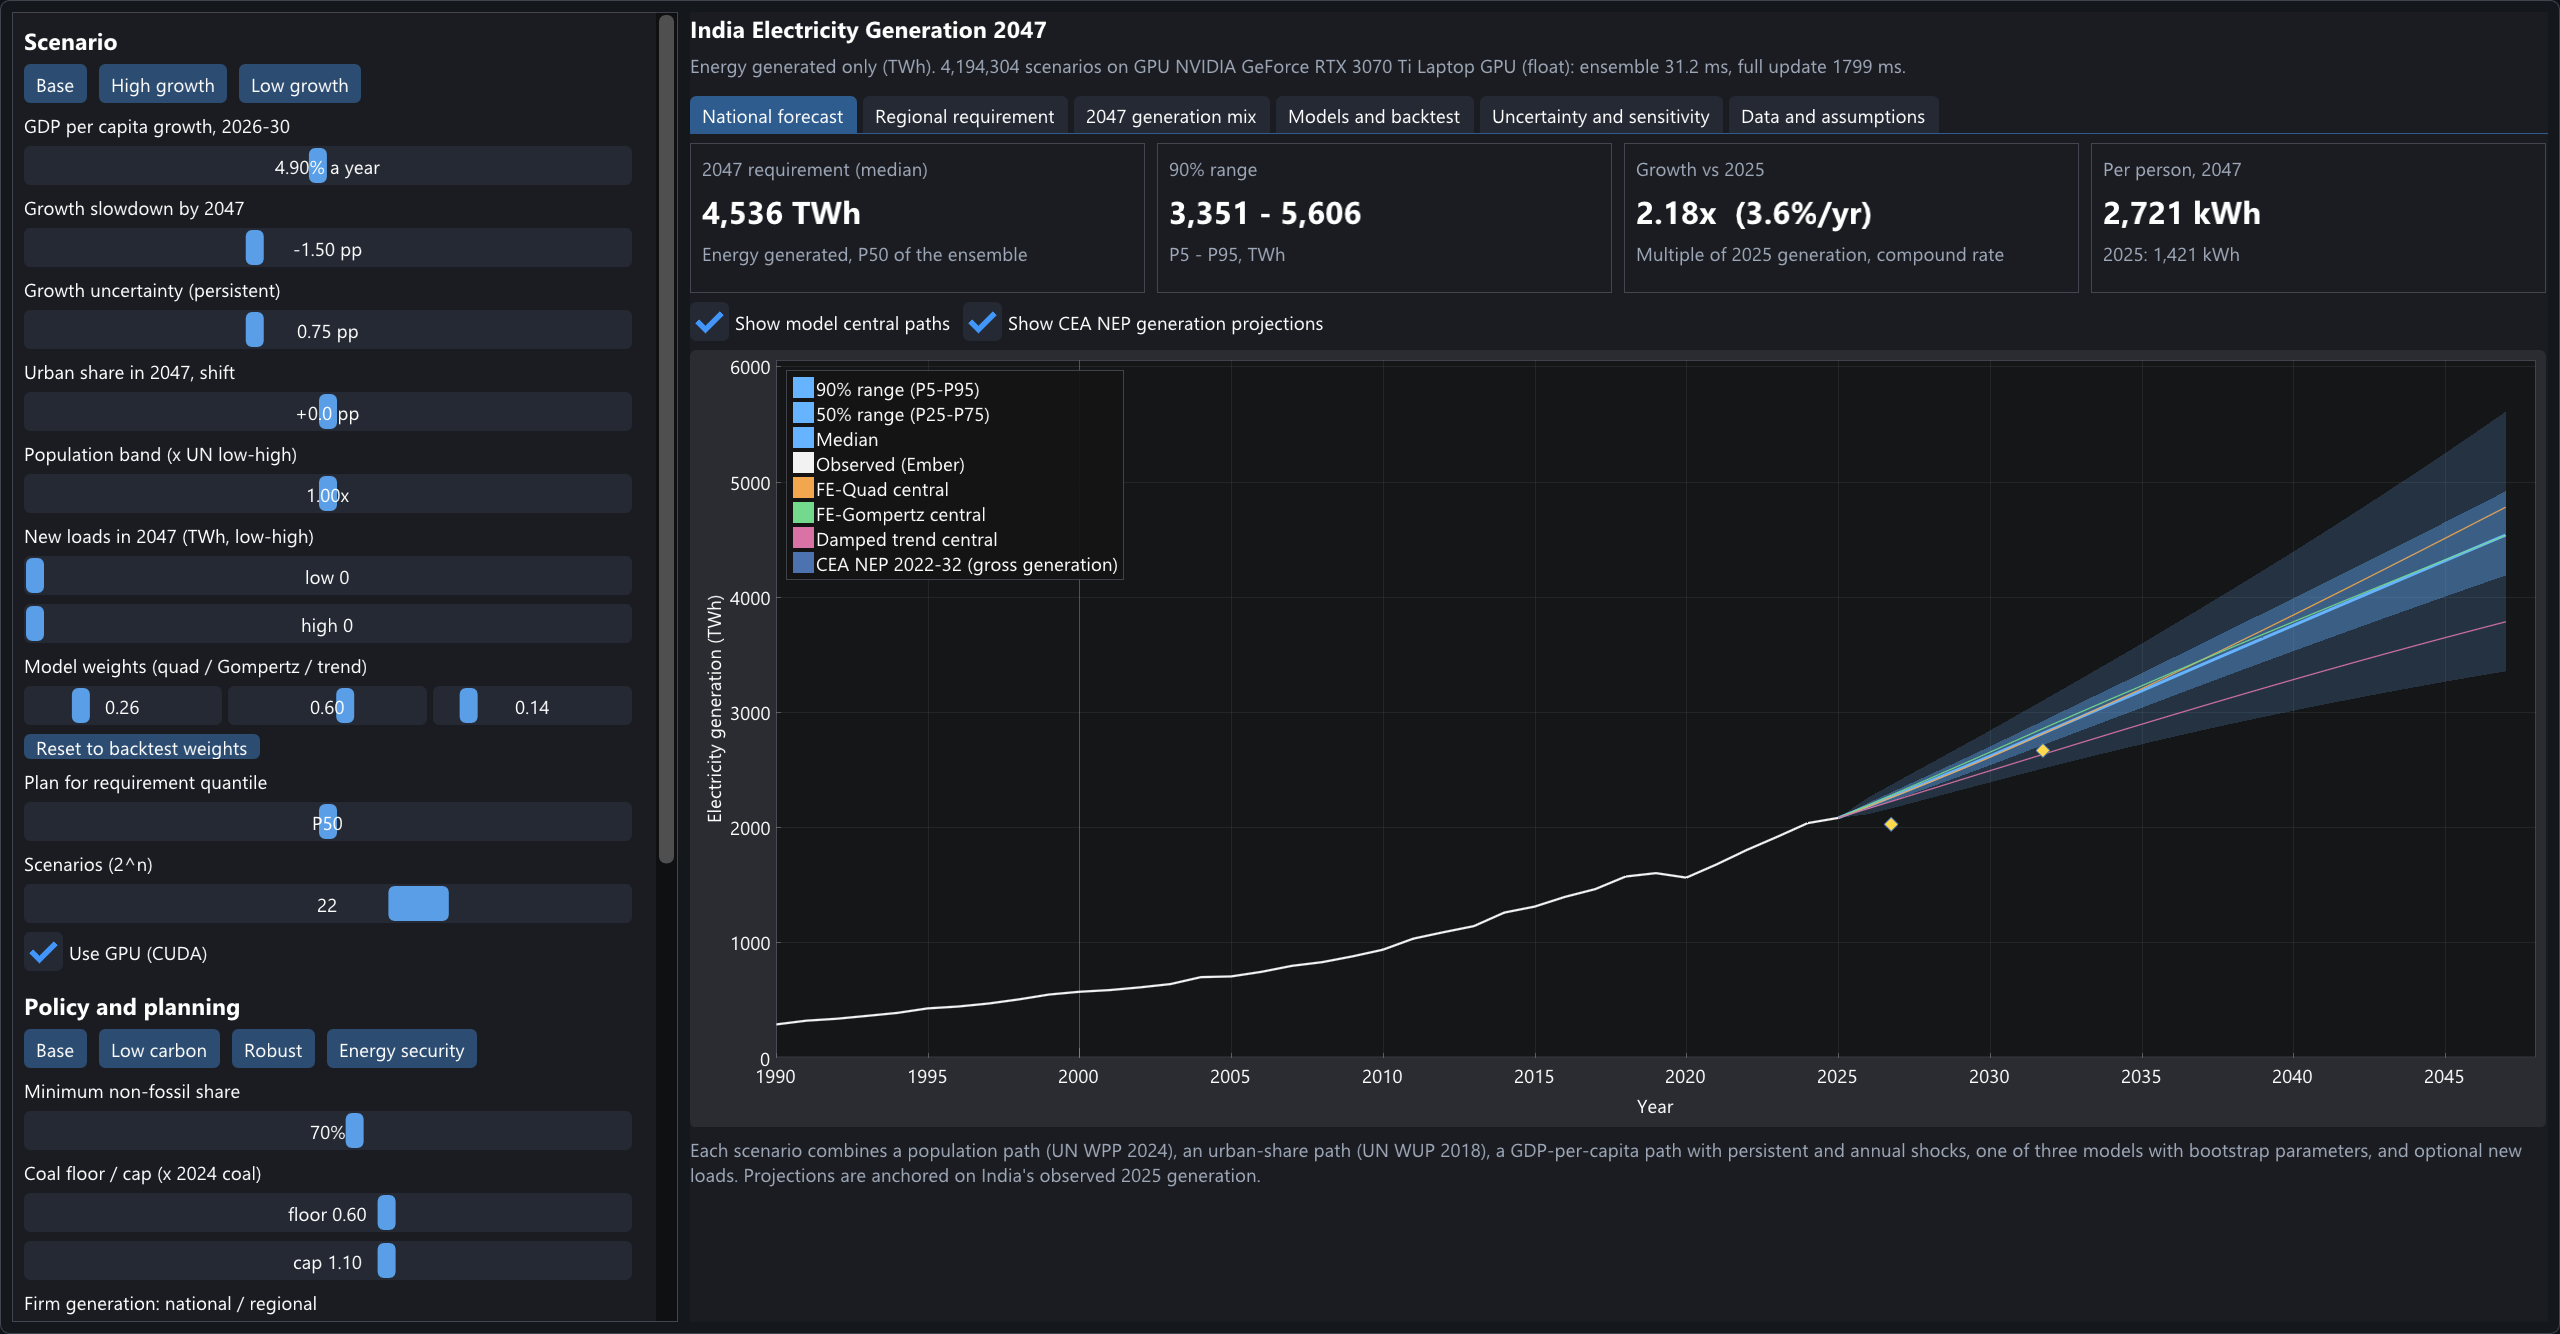
\includegraphics[width=\linewidth]{../img/1_national_forecast.png}
\column{\gB\textwidth}
\vspace{1mm}
{\fontsize{8.5}{10.5}\selectfont
\textbf{\color{navy}Six views}\par\vspace{1mm}
National fan chart with the CEA benchmark\\
Regional requirement\\
2047 mix: least cost vs resource score\\
Models and backtest\\
Uncertainty and sensitivity\\
Data and assumptions\par\vspace{2mm}
\textbf{\color{navy}One-click presets}\par\vspace{1mm}
Core: India-only (primary), cross-country (check)\\
Growth: base, high, low\\
Policy: base, low carbon, robust, energy security}
\end{columns}
\evidence{Native C++ application (Dear ImGui, ImPlot, OpenGL), same engine as all results; screenshot \texttt{docs/img/1\_national\_forecast.png} \cite{e47_repo}.}
\note{%
\textbf{Demo script (2 minutes).} (1) Show the fan chart with NPP history and the CEA diamonds. (2) Move income growth by 1.5 points and watch the 2047 median move by about a quarter. (3) Switch the core to the cross-country check and back. (4) Switch the policy preset from Base to Robust and point to unmet energy, CO$_2$ and cost.\par\medskip
\textbf{Fallback.} If screen sharing lags, use the images in \texttt{docs/img/}.}
\end{frame}

% ===================================================================== 17
\begin{frame}{What we recommend, and what comes next}
\begin{columns}[T,onlytextwidth]
\column{\gA\textwidth}
\card{\linewidth}{\fontsize{8.2}{10.1}\selectfont
\textbf{\color{navy}Recommendations for India's 2047 plan}\par\vspace{1mm}
\begin{enumerate}\setlength{\itemsep}{0.3mm}
\item \textbf{Plan for growth, not one number}: income growth moves 2047 by $-$24\% to +32\%; update the plan as NPP data arrive.
\item \textbf{Unlock land}: 35\% of solar potential usable closes the median gap; P90 needs 45--55\%.
\item \textbf{Build faster}: 2.5--3.5$\times$ India's record annual addition.
\item \textbf{Serve the North, South and North-East}: their need grows beyond what they make today.
\item \textbf{Decarbonise the coal that remains}: 23.5\% of 2047 generation and 1,114\,Mt CO$_2$ in the robust plan, a large opportunity for carbon capture.
\end{enumerate}}
\column{\gB\textwidth}
{\fontsize{8.2}{10}\selectfont
\textbf{\color{navy}Before the final}\par\vspace{1mm}
Organiser ruling on the urbanisation prior and the captive layer.\\[0.8mm]
Regional renewable generation (not on NPP).\\[0.8mm]
Hourly adequacy check with NPP Merit profiles.\\[0.8mm]
Industrial-demand layer for steel and aluminium regions.\par\vspace{2.5mm}
\textbf{\color{navy}Limitations we state openly}\par\vspace{1mm}
Regional requirement is modelled, not observed; history includes supply shortages; annual energy only; 2047 costs follow one published path.}
\end{columns}
\evidence{Recommendations follow from slides 10--14: \texttt{outputs/sensitivity\_2047.csv}, \texttt{tornado.csv}, \texttt{presets.csv}, \texttt{p90\_levers.csv} \cite{e47_repo}; NPP coverage \cite{npp_dashboard,npp_merit}; assumptions: \texttt{docs/assumptions\_and\_uncertainty.md}.}
\note{%
\textbf{Why recommendation 5 matters to ExxonMobil.} Even the robust plan keeps 23.5\% coal in 2047 because the existing fleet is young (coal floor 50\% of 2024 output). The 1,114\,Mt of CO$_2$ that remains is concentrated at large stations, which is where carbon capture and storage is most practical.\par\medskip
\textbf{Rulings requested.} (1) May a literature prior (urbanisation) enter the core, given that urban share is in neither dataset? Our $\gamma = 0$ run (4,647\,TWh) is ready if not. (2) May captive generation be reported as a separate layer?\par\medskip
\textbf{Data gaps.} NPP has no renewable generation after FY2023-24 except all-India Merit solar and wind from 18 September 2025, and none by region.}
\end{frame}

% ===================================================================== 18
\begin{frame}[allowframebreaks]{References}
\printbibliography[heading=none]
\end{frame}

% ===================================================================== backup
\appendix
\begin{frame}{Backup: core forecast and independent check}
\vspace{1mm}
{\fontsize{7.8}{9.5}\selectfont
\renewcommand{\arraystretch}{1.25}
\setlength{\tabcolsep}{4pt}
\begin{tabular}{@{}>{\raggedright\arraybackslash}p{3.7cm}>{\raggedright\arraybackslash}p{3.6cm}rrrr@{}}
\toprule
Model & Scope (base year) & Base & 2047 P5 & \textbf{2047 median} & 2047 P95\\
\midrule
\textbf{India-only (core)} & NPP utility generation (FY2023-24) & 1,698 & 3,248 & \textbf{4,894} & 7,526\\
India-only + captive layer & utility + captive, CEA share held & 1,922 & 3,676 & \textbf{5,540} & 8,519\\
Cross-country panel (check) & Ember total incl.\ captive (calendar 2025) & 2,080 & 3,348 & \textbf{4,528} & 5,610\\
\midrule
India-only, $\gamma = 0$ & two datasets only & 1,698 & 2,973 & 4,647 & 7,438\\
India-only, elasticity decline 0.2 & saturation as in the panel & 1,698 & 3,139 & 4,367 & 5,980\\
\bottomrule
\end{tabular}\par}
\vspace{2mm}
{\fontsize{8}{9.8}\selectfont
The check lands inside the core's range, 18\% below the captive-inclusive core. The gap is the elasticity: 153 countries imply 0.44--0.57 at India's income, falling with income; India's own data give 0.78--0.90. A decline of 0.2 per unit of log income brings the core to 4,367\,TWh, close to the check.\par}
\evidence{\texttt{outputs/core\_comparison.csv}, \texttt{sensitivity\_2047.csv}, \texttt{forecast\_secondary\_cross\_country.csv} \cite{e47_repo}; check data \cite{ember_yearly,wb_wdi}; captive \cite{cea_general_review_2025}; cross-country elasticities: \texttt{docs/methodology.md}, section 3.}
\note{Use this slide if asked why two numbers exist. The core is the only forecast; the check uses non-core data and answers one question: does an independent method land in the same range? It does, and the gap is explained by one parameter.}
\end{frame}

\begin{frame}{Backup: assumptions and their controls}
{\fontsize{7.3}{8.7}\selectfont
\renewcommand{\arraystretch}{1.1}
\begin{tabular}{@{}>{\raggedright\arraybackslash}p{3.4cm}>{\raggedright\arraybackslash}p{5.3cm}>{\raggedright\arraybackslash}p{4.9cm}@{}}
\toprule
Assumption & Value & Basis\\
\midrule
Income elasticity & bootstrap mix, median 0.870 (90\%: 0.747--0.950) & NPP and organiser data \cite{npp_dashboard,organiser_dataset}\\
Excess urbanisation $\gamma$ & $N(1.0,\,0.5)$ truncated at 0; $\kappa = 0.092$ & \cite{liddle2013population,shahbaz2016role,holtedahl2004residential}\\
Income growth per person & 4.95\%/yr to 2030 (s.d.\ 1.5\%), slowing 1.5\,pp by 2047 & organiser GSDP, FY2012-13 to FY2023-24 \cite{organiser_dataset}\\
Base year & FY2023-24, anchor shift $-$0.043 log points & 3-year mean residual, \texttt{india\_fit.csv}\\
Population, urban share & UN WPP 2024 medium; UN WUP 2018 change, $\pm$2\,pp & \cite{un_wpp2024,un_wup2018}\\
State income convergence & 0.021/yr (s.e.\ 0.011) & \cite{organiser_dataset,barro1992convergence}\\
Captive layer & 13.2\% of utility generation, held & \cite{cea_general_review_2025} (Table 1.6)\\
Usable resource & 25\% of solar and wind, 70\% of hydro & \cite{mnre_restats_2425,cea_hydro_status}\\
Coal fleet & floor 60\% of 2024; national cap 110\% & \cite{cea_nep2023}\\
Build rates & $\le$ 2025 + 22 yr $\times$ 2 $\times$ record annual increase & \cite{ember_yearly}\\
Costs 2047; corridors & IEA India LCOE, SECI tenders; 2$\times$ 2032 plan at 60\% & \cite{iea_weo2025,seci_auctions,cea_nep_vol2}\\
\bottomrule
\end{tabular}}
\evidence{Full list with sources and the dashboard control for each: \texttt{docs/assumptions\_and\_uncertainty.md}; values \texttt{outputs/india\_fit.csv} \cite{e47_repo}.}
\note{Every row is adjustable in the dashboard and documented with its source. Build-rate records use Ember generation history (outside the core, as a limit, not a forecast input).}
\end{frame}

\begin{frame}{Backup: twelve futures, four policies}
{\fontsize{7.2}{8.8}\selectfont
\renewcommand{\arraystretch}{1.08}
\setlength{\tabcolsep}{4.5pt}
\begin{tabular}{@{}llrrrrrr@{}}
\toprule
Scenario & Policy & Median TWh & Non-fossil & CO$_2$ Mt & Cost bn USD & Unmet at median & Unmet at P90\\
\midrule
Base & Base & 4,894 & 70.0\% & 1,364 & 233 & 28 & 1,958\\
Base & Low carbon & 4,894 & 80.0\% & 865 & 211 & 47 & 1,979\\
Base & \textbf{Robust} & 4,894 & \textbf{76.5\%} & \textbf{1,114} & \textbf{188} & \textbf{0} & \textbf{1,067}\\
Base & Energy security & 4,894 & 70.0\% & 1,366 & 233 & 30 & 1,958\\
High growth & Base & 7,088 & 70.0\% & 1,416 & 240 & 2,217 & 5,060\\
High growth & Robust & 7,088 & 75.0\% & 1,396 & 256 & 1,326 & 4,169\\
Low growth & Base & 3,516 & 77.4\% & 772 & 134 & 0 & 0\\
Low growth & Robust & 3,516 & 81.2\% & 643 & 125 & 0 & 0\\
\bottomrule
\end{tabular}}
\vspace{2mm}
{\fontsize{8}{9.8}\selectfont\color{ink2}High growth: income growth 1.5 points above history, urban share +3 points, 100--300\,TWh of new loads. Low growth: 1.5 points below, urban share $-$2 points.\par}
\evidence{\texttt{outputs/presets.csv} (all twelve combinations) \cite{e47_repo}.}
\note{Under low growth every policy is adequate and the robust policy is cheapest and cleanest. Under high growth no preset meets the median: 7,088\,TWh needs the land and build-rate levers pushed well beyond the robust settings. Energy security under high growth is infeasible at P90.}
\end{frame}

\begin{frame}{Backup: data limits we work around}
{\fontsize{8}{9.8}\selectfont
\renewcommand{\arraystretch}{1.25}
\begin{tabular}{@{}>{\raggedright\arraybackslash}p{4.8cm}>{\raggedright\arraybackslash}p{4.3cm}>{\raggedright\arraybackslash}p{4.6cm}@{}}
\toprule
Limit & Effect & What we do\\
\midrule
NPP all-India series ends FY2023-24; RES after that only as Merit solar and wind from Sep 2025 & No renewable generation for FY2024-25; holdout needs an estimate & Extend NPP RES at its FY2018-23 growth (14.1\%/yr); report it\\
No regional RES on NPP & Today's regional shares are conventional only & Compare shares, not levels; flag the bias\\
Urban share in neither dataset & Cannot be estimated separately from income & Literature prior $\gamma$; $\gamma = 0$ run shown ($-$5\%)\\
Organiser GSDP: 2011 price-base break; 2024 incomplete & Spurious jump in 2011 & Impute 2011 growth (4.27\%); drop 2024\\
Captive plants outside NPP & Utility scope only & Separate layer at 13.2\%\\
History includes supply shortages & Elasticity may be high & State it; elasticity-decline case\\
\bottomrule
\end{tabular}}
\evidence{NPP coverage, \texttt{data/raw/npp/SOURCES.md} \cite{npp_dashboard,npp_18col,npp_merit}; organiser data \cite{organiser_dataset}; captive plants \cite{cea_general_review_2025}; \texttt{outputs/india\_fit.csv}, \texttt{holdout.csv}, \texttt{sensitivity\_2047.csv} \cite{e47_repo}.}
\note{These are the roadblocks reported at the midpoint review. Each has a stated workaround and a switch in the model, so the jury can see its effect.}
\end{frame}

\end{document}
